% !TEX root = ../../main.tex

\subsection{Characterisation of trends}\label{def:trends}

The graphs in \autoref{def:fgr:tga-defects} summarize the 
trends in missing linker defects as calculated through 
the TGA plateau at \SI{420}{\degreeCelsius}. The DMF leached samples,
due to the multiple datapoints with different acid concentrations
show the clearest influence of this variable on defect
generation. Even small amounts of modulator leads to the decrease of 
the linker-to-node ratio, but the increase in concentration stops 
having an effect at around 20:1 equivalents. It is likely that
the trends are similar with other solvents, even if less 
datapoints are available.

\begin{figure}[htb]
    \centering

    \begin{subfigure}{0.45\linewidth}
        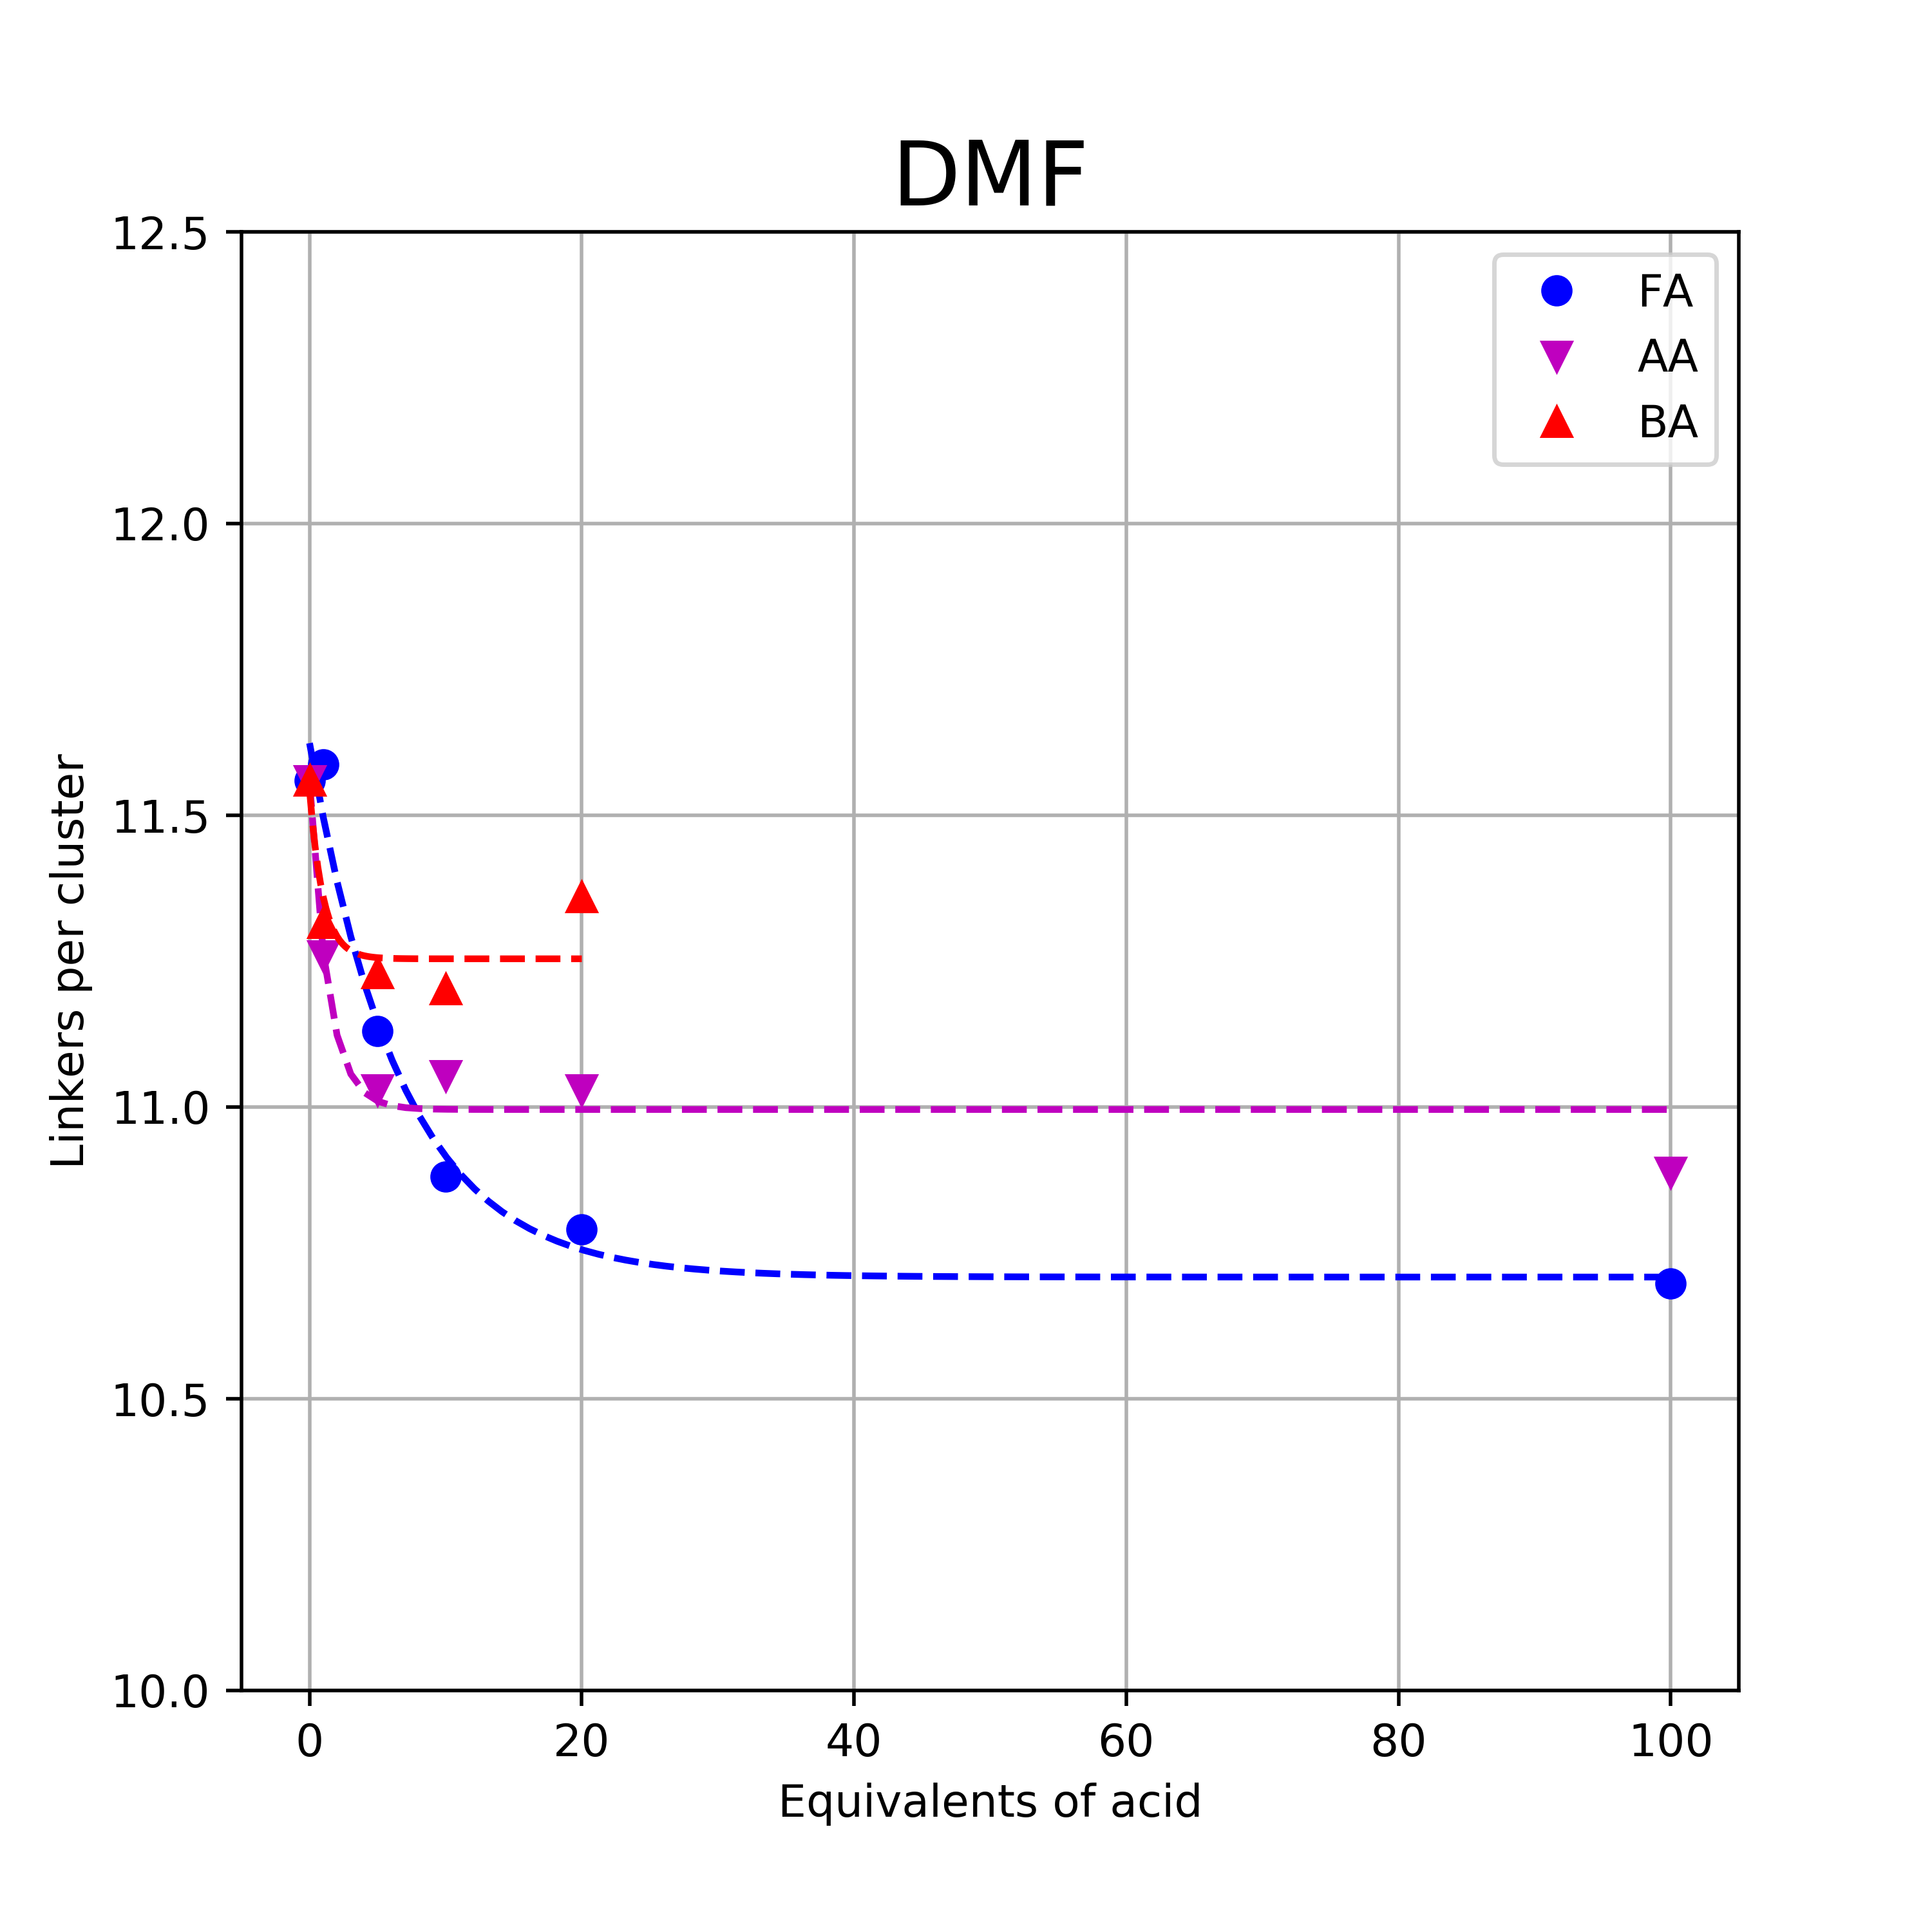
\includegraphics[width=\textwidth]{tga/DMF-def-overview}%
        \label{def:fgr:tga-dmf-linkers}
    \end{subfigure}
    \begin{subfigure}{0.45\linewidth}
        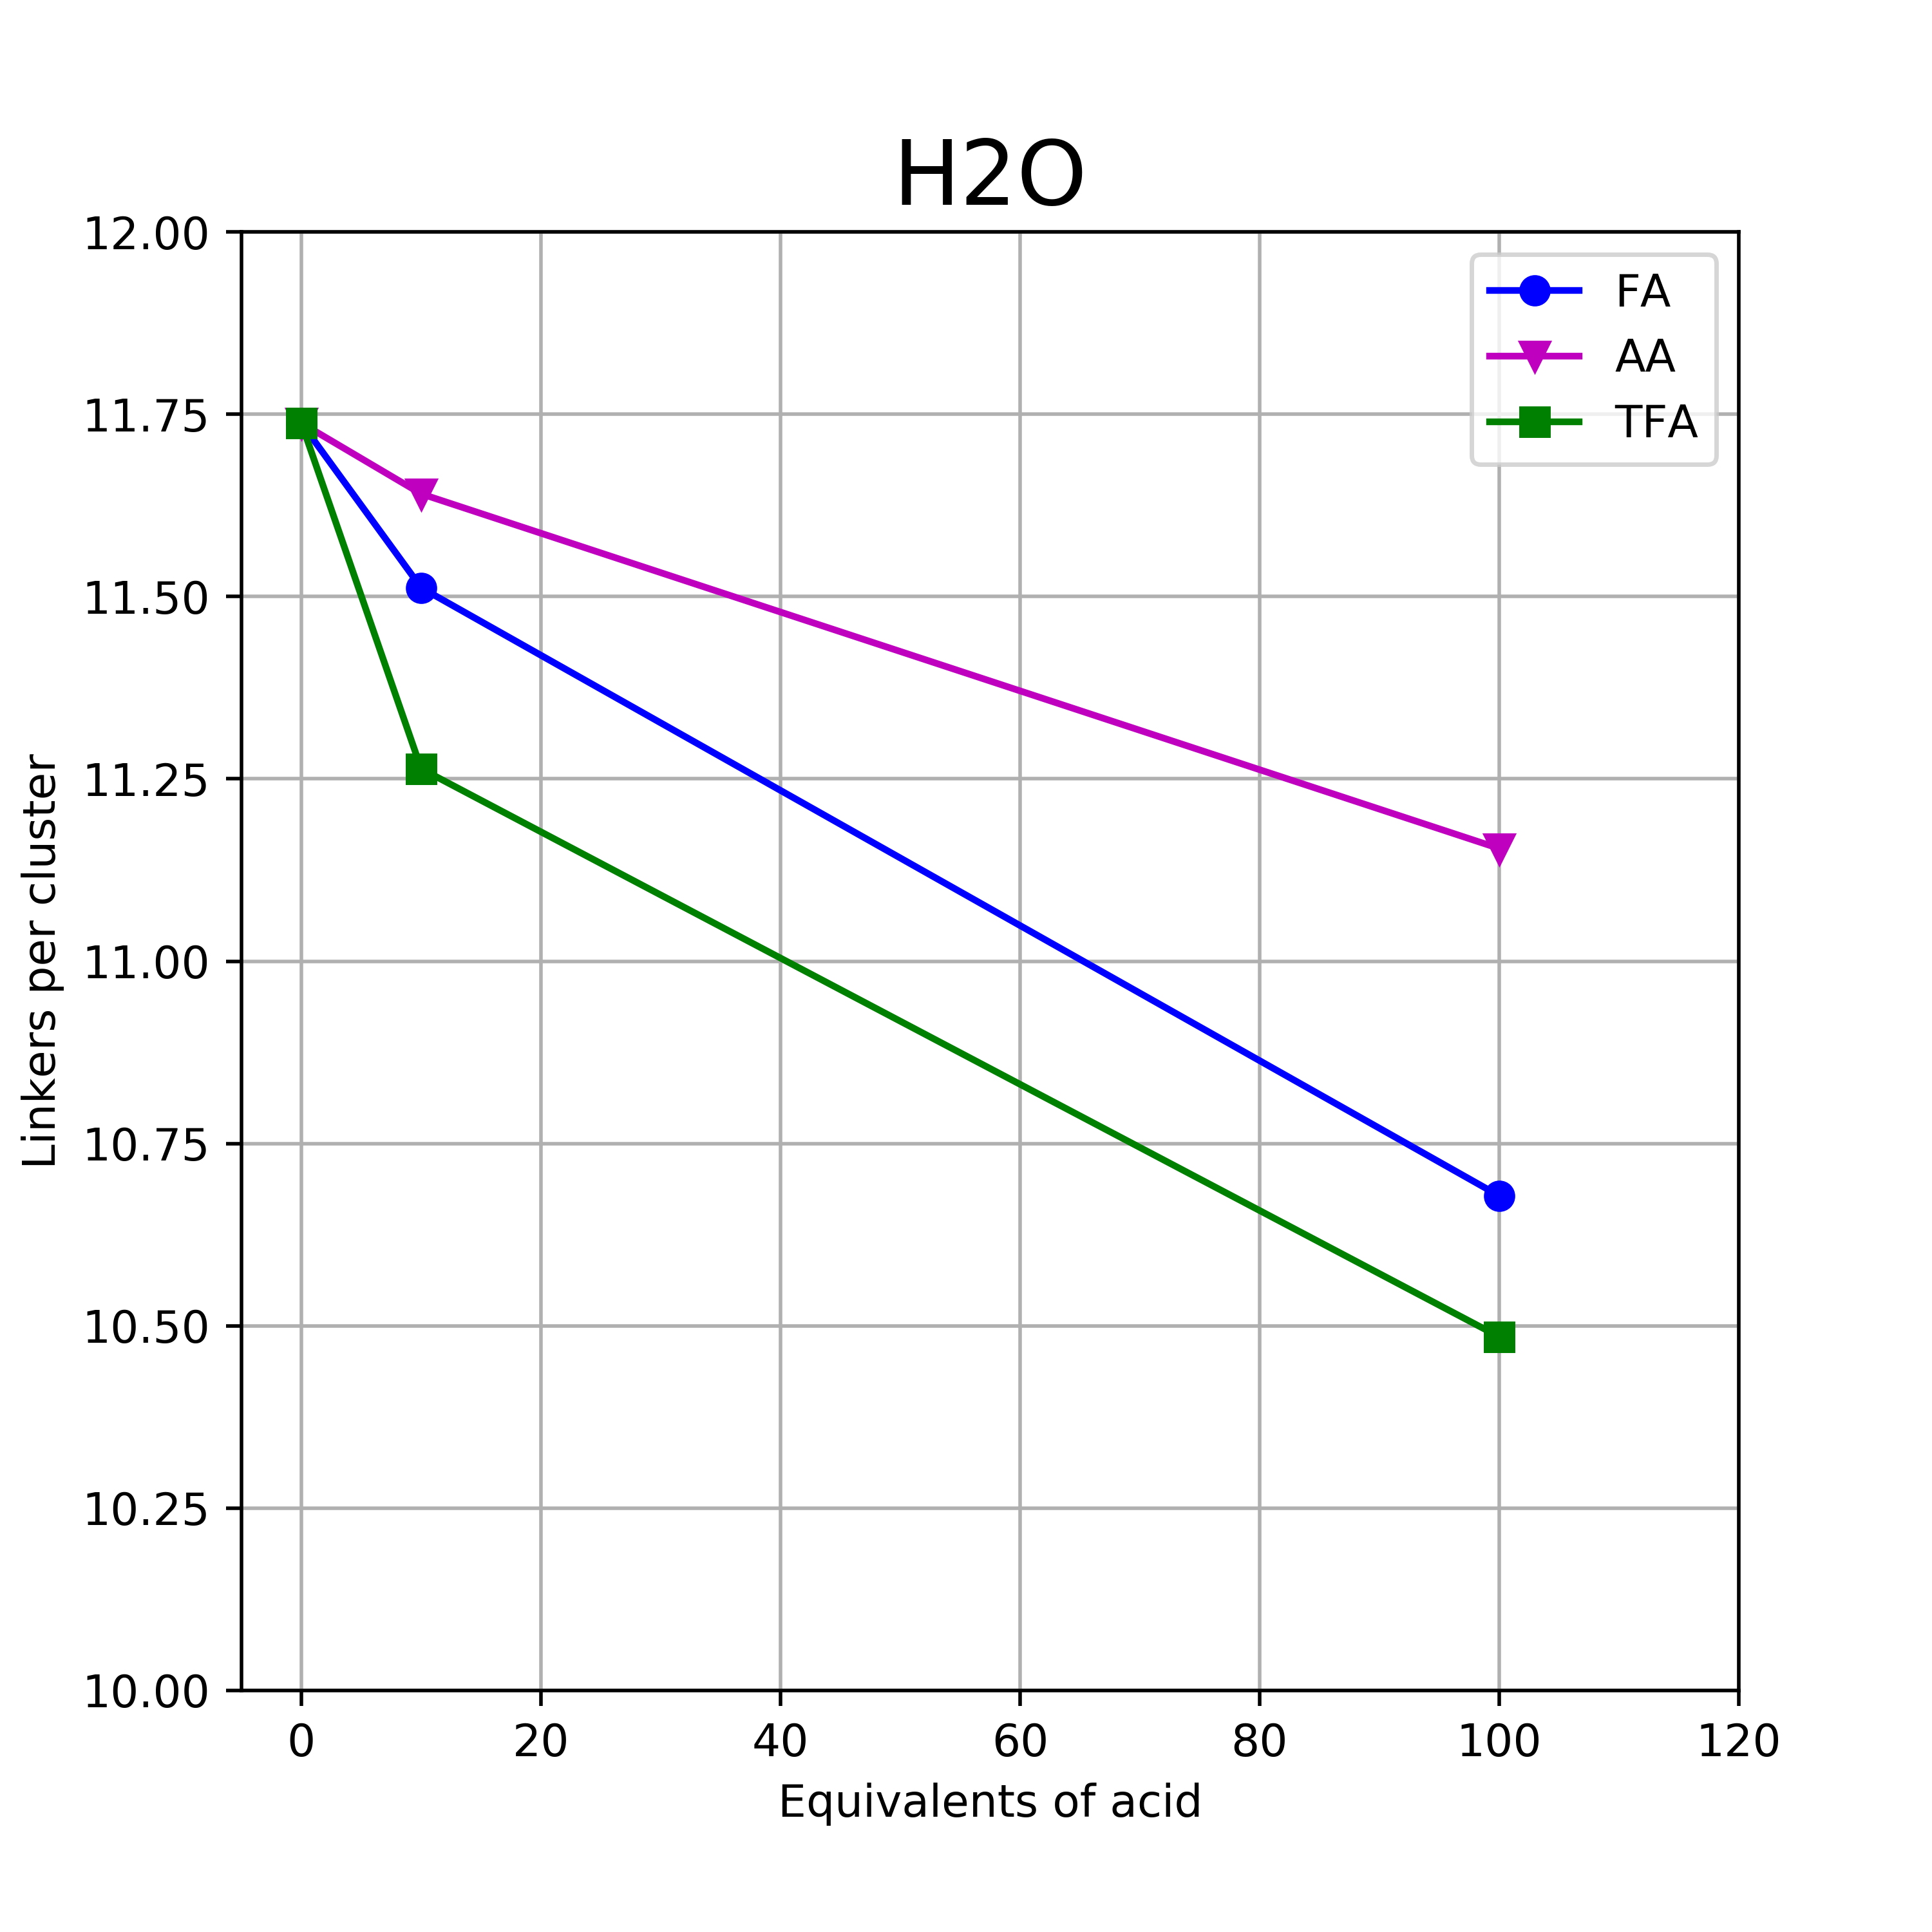
\includegraphics[width=\textwidth]{tga/H2O-def-overview}%
        \label{def:fgr:tga-h2o-linkers}
    \end{subfigure}

    
    \begin{subfigure}{0.45\linewidth}
        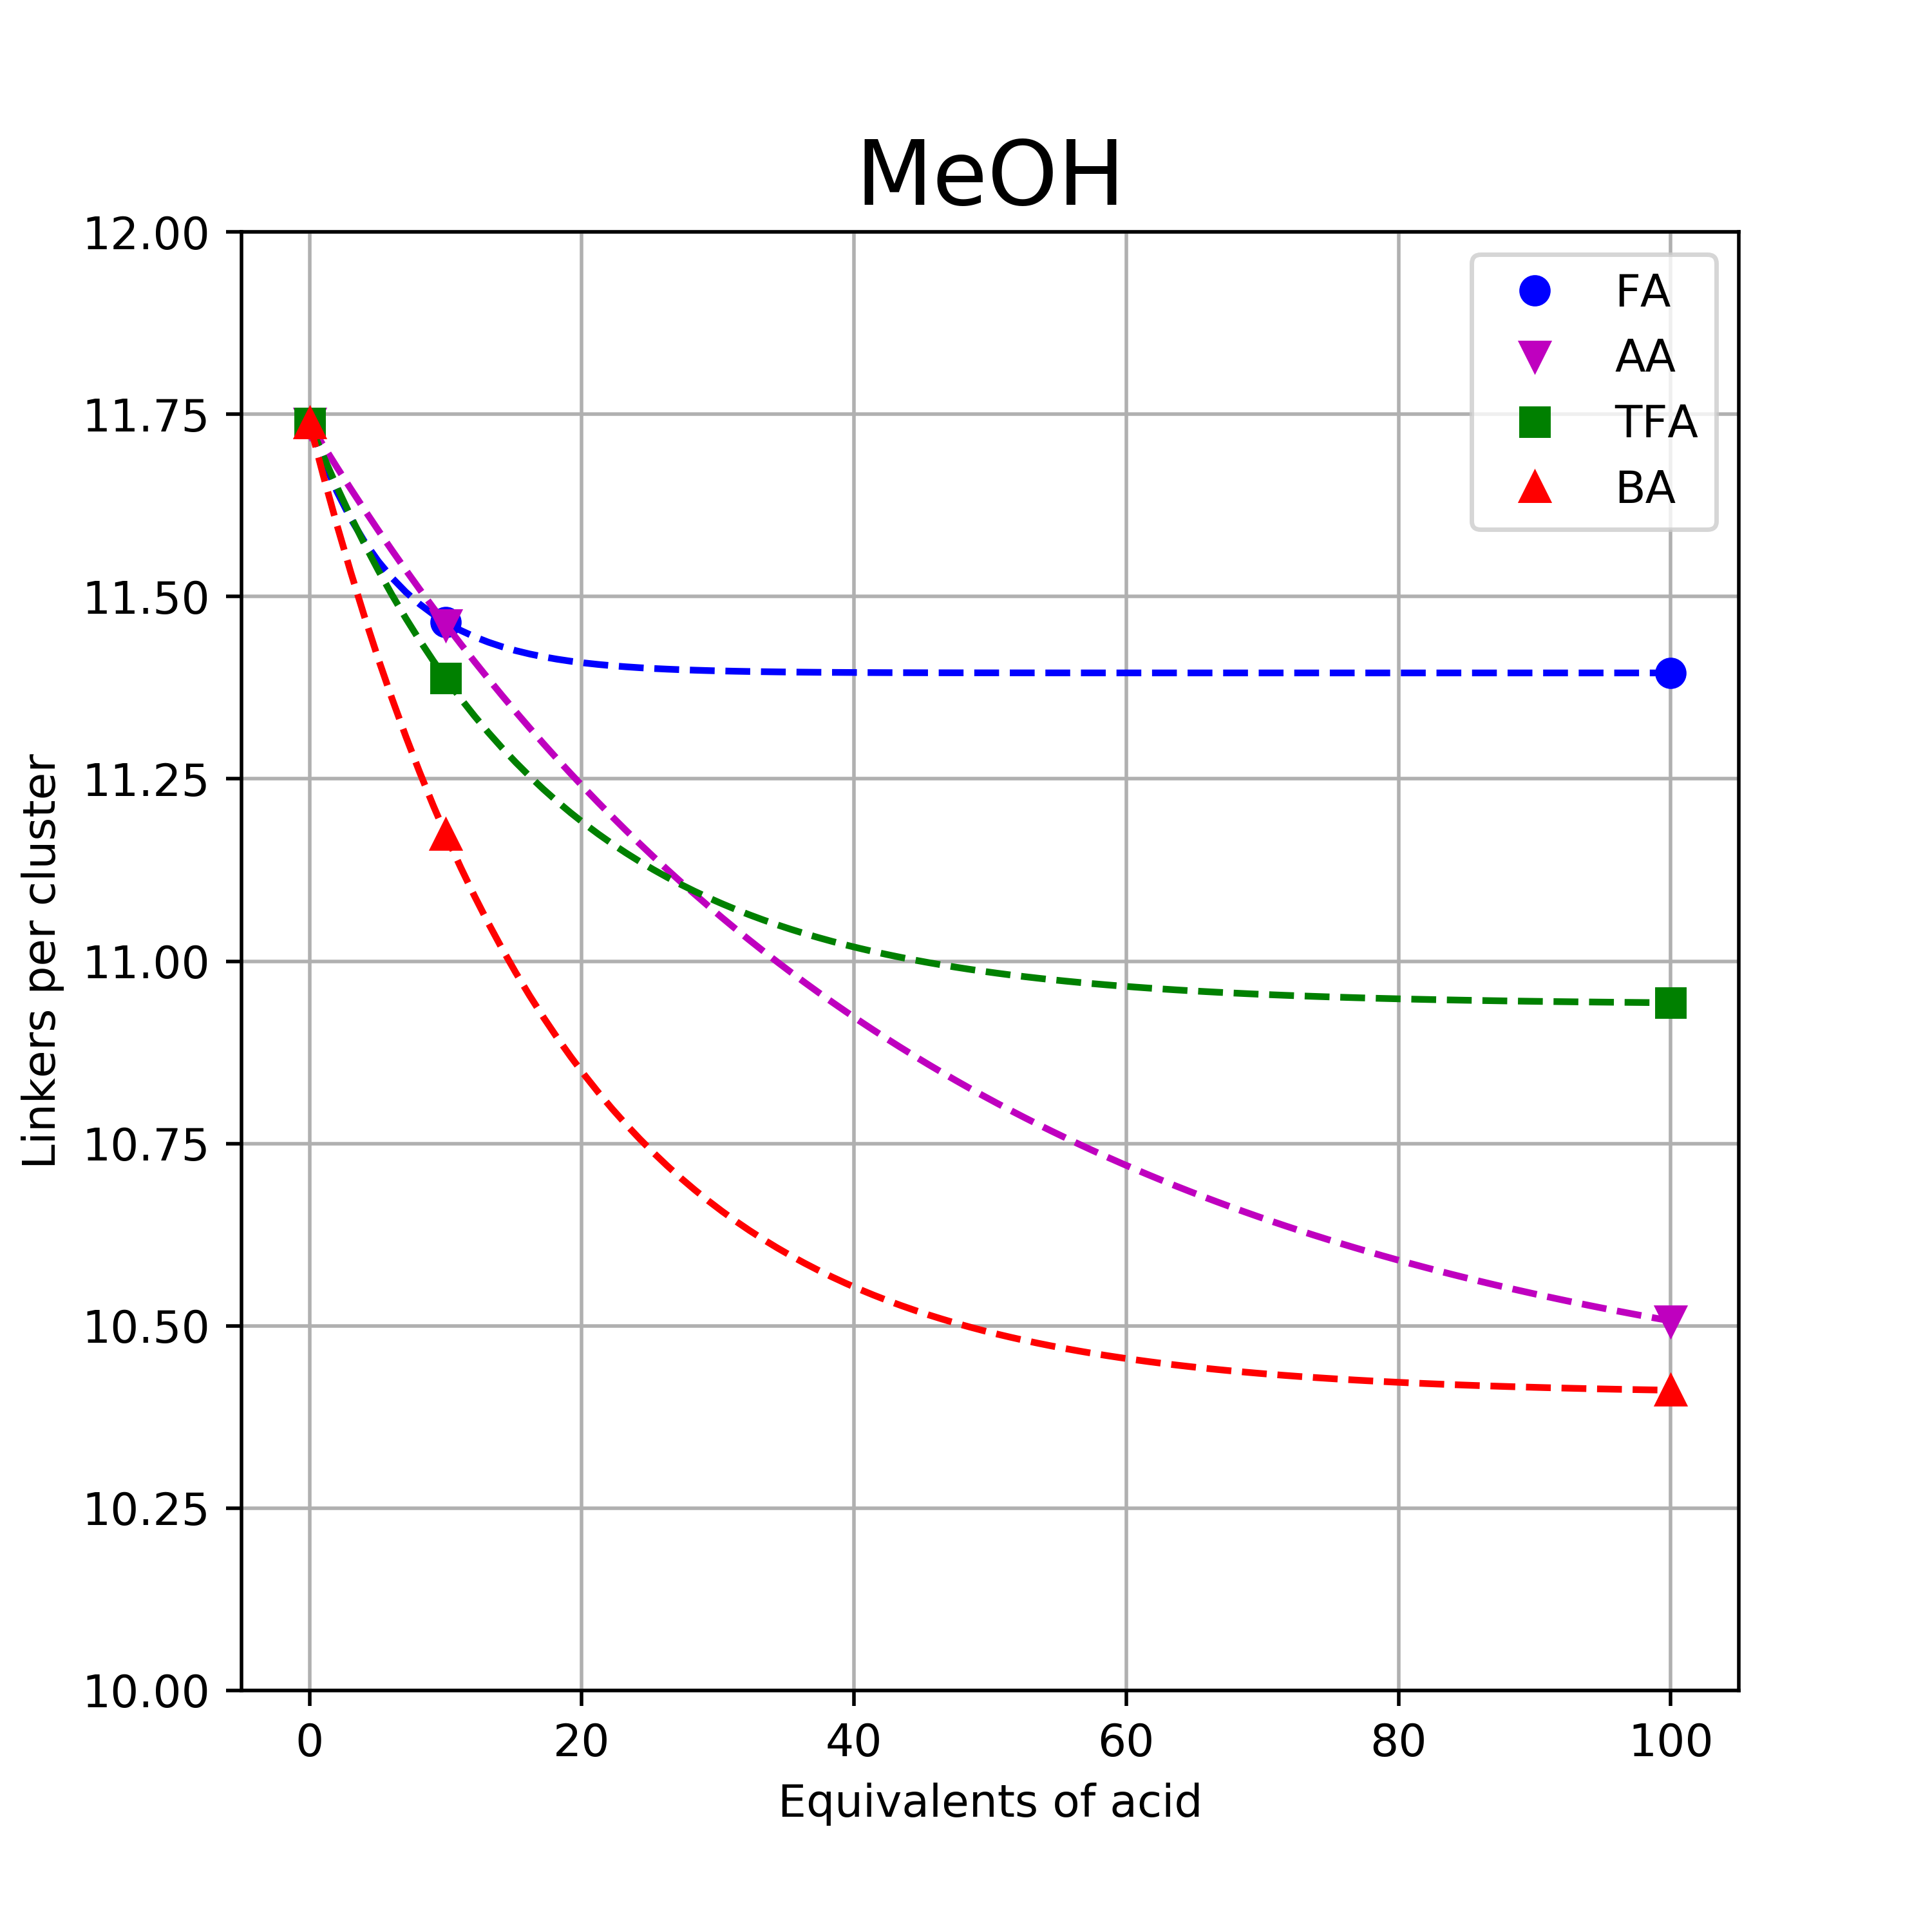
\includegraphics[width=\textwidth]{tga/MeOH-def-overview}%
        \label{def:fgr:tga-meoh-linkers}
    \end{subfigure}
    \begin{subfigure}{0.45\linewidth}
        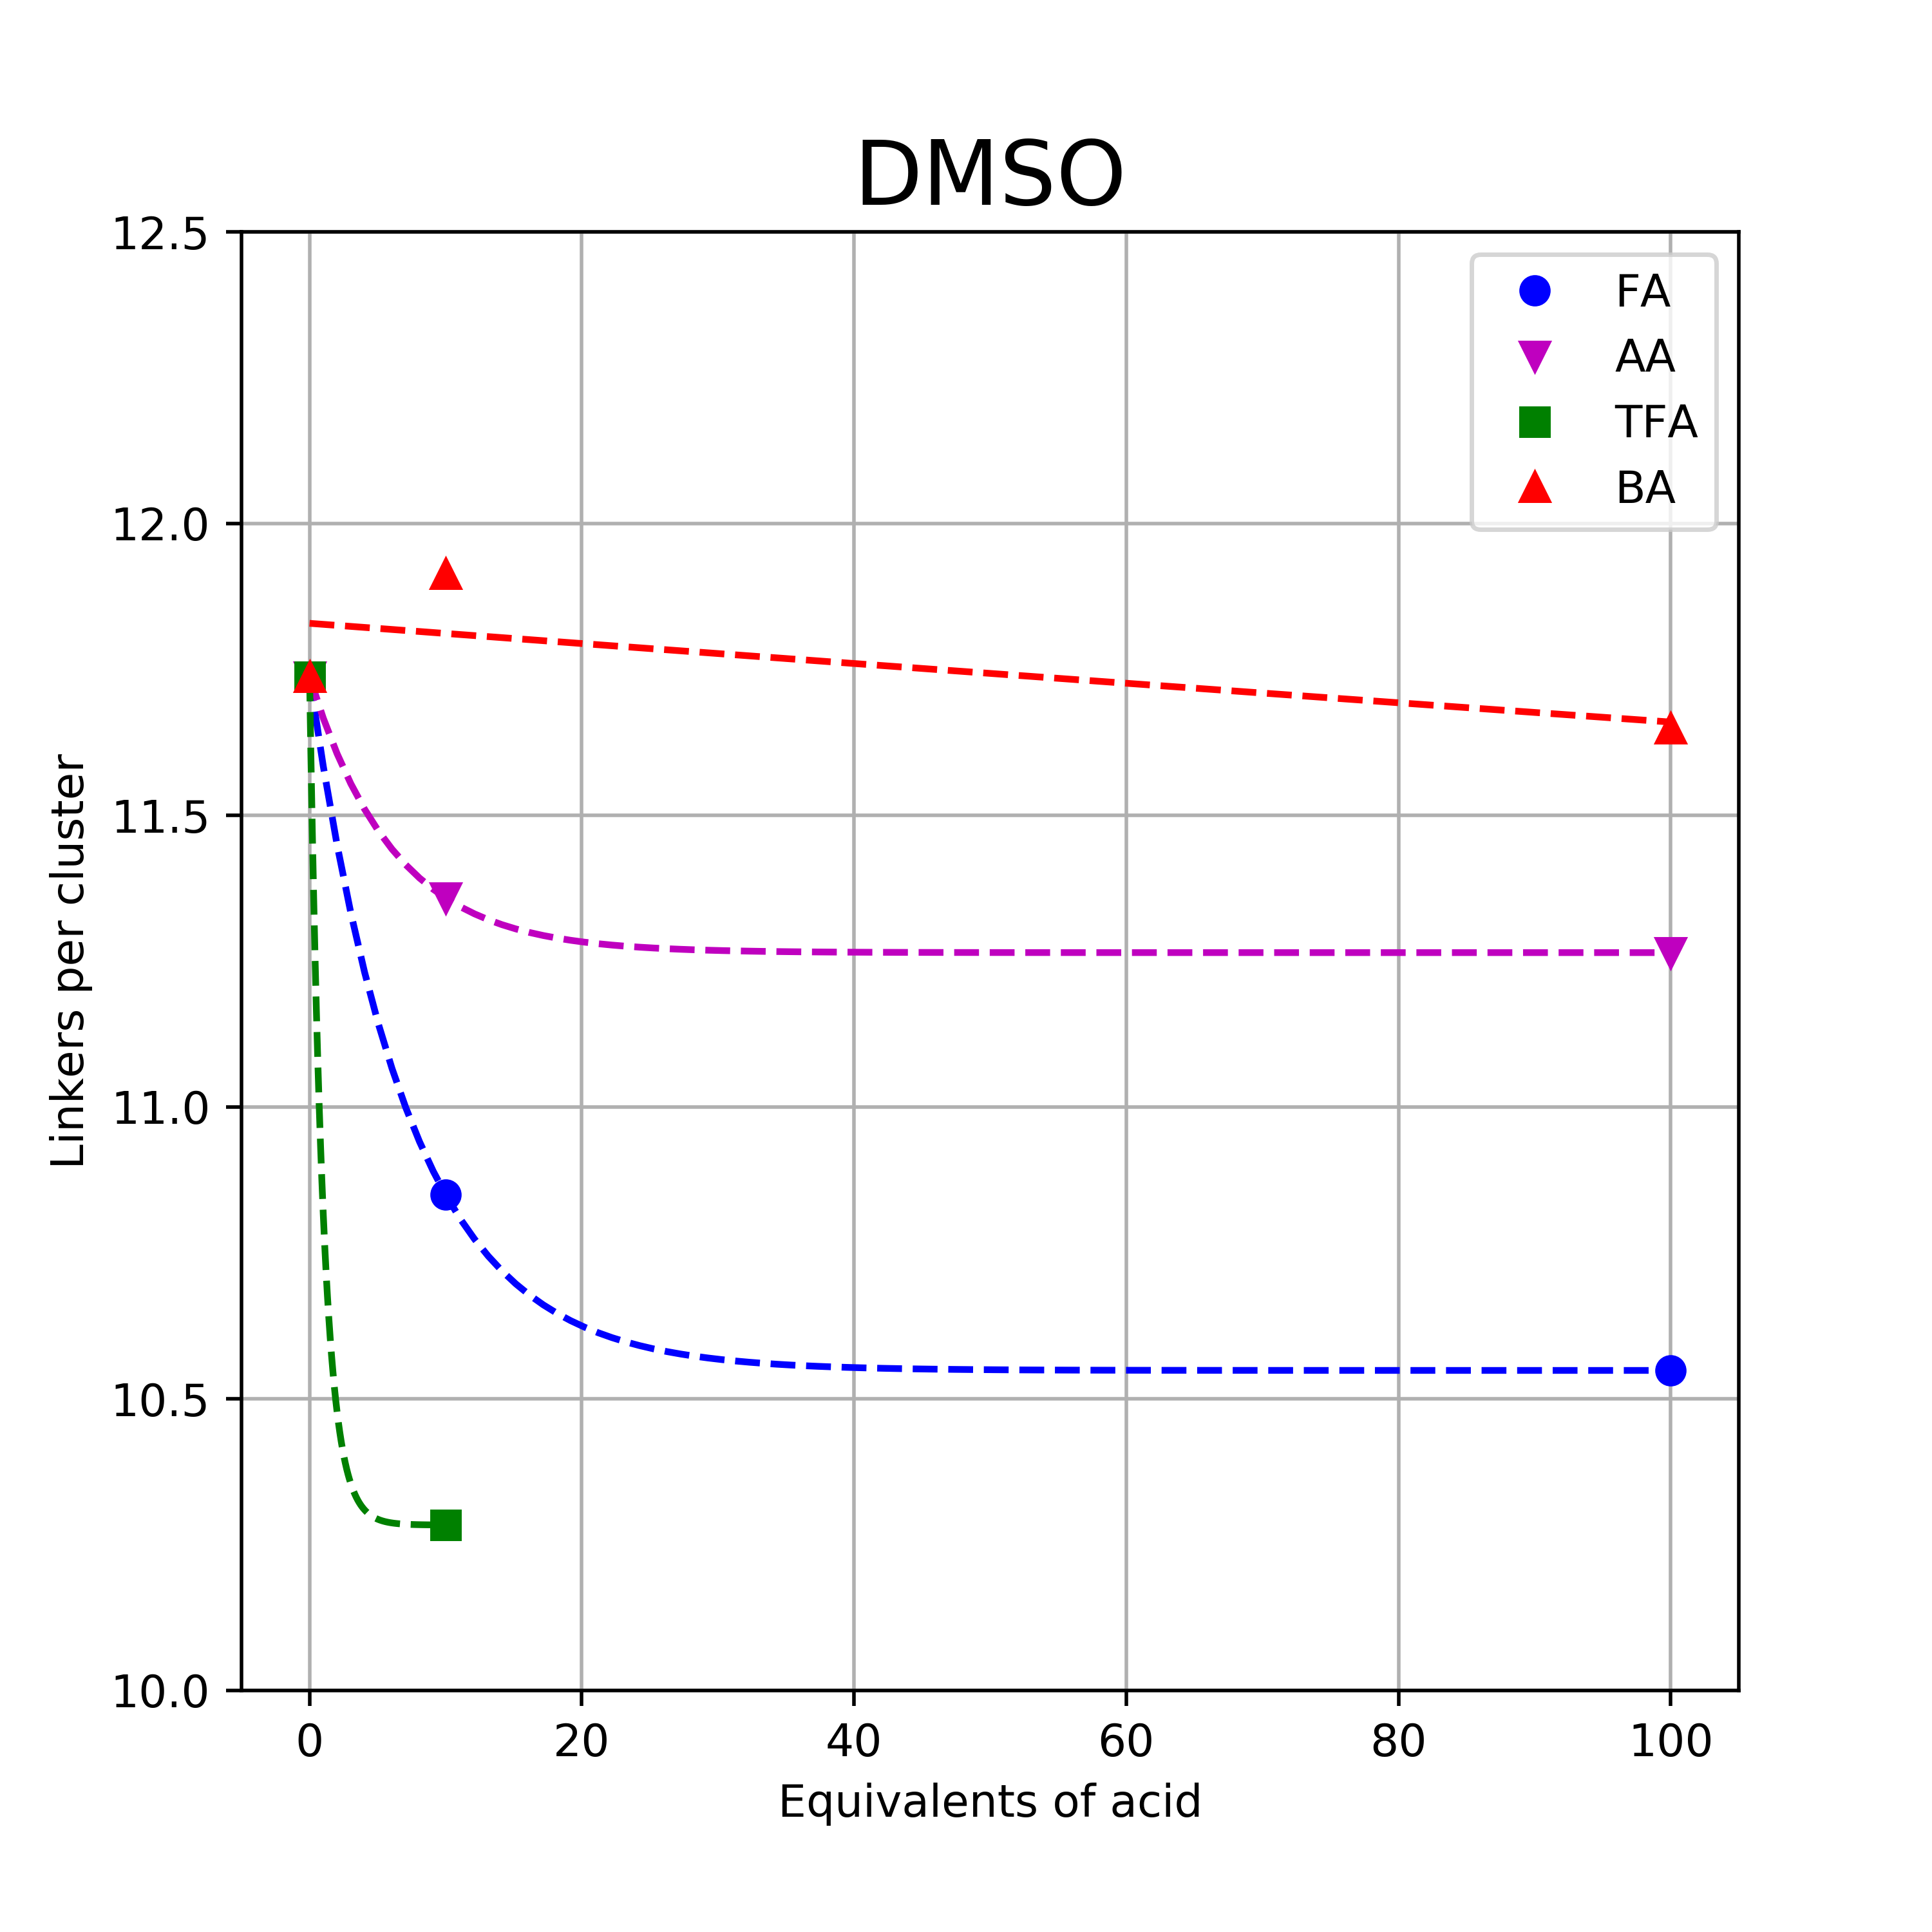
\includegraphics[width=\textwidth]{tga/DMSO-def-overview}%
        \label{def:fgr:tga-dmso-linkers}
    \end{subfigure}

    \caption{Calculated linker-to-node ratio from the TGA curve 
    normalized mass at \SI{420}{\degreeCelsius} for (a) DMF 
    (b) \ce{H2O}, (c) \ce{MeOH} and (d) DMSO leached samples.
    A ratio of 12 to 1 corresponds to a completely defect-free
    structure. An exponential decay trendline is fitted to 
    each set of points.}%
    \label{def:fgr:tga-defects}
    
\end{figure}


When DMF is used as a solvent, the resulting leached samples 
have a 

Since multiple concentrations of modulator were used only with 
DMF, inly a general trend is available.